\documentclass[12pt,a4paper]{article}
\usepackage{../lecture-notes/vkCourseML}
\usepackage{lipsum}
\usepackage{indentfirst}
\title{Машинное обучение, ФКН ВШЭ\\Семинар №5}
\author{}
\date{}
\begin{document}
	\maketitle
	\section{AUC-ROC}
	\par На лекции мы познакомились с такой важной метрикой качества бинарной классификации, как площадь под ROC-кривой (AUC-ROC). Напомним её определение. Рассмотрим задачу бинарной классификации с метками классов $\mathbb{Y} = \{ -1, +1\},$ и пусть задан некоторый алгоритм $b(x)$, позволяющий вычислять оценку принадлежности объекта $x$ положительному классу. AUC-ROC позволяет оценивать качество классификации для семейства алгоритмов следующего вида:
	$$a(x; t) = \begin{cases}
		-1, \, b(x) \le  t,\\
		+1, \, b(x) > t,
	\end{cases}$$
	т.е. алгоритмов, присваивающих метки объектам в соответствии с оценками $b(x)$, отсекая их по некоторому порогу $t$. Каждый алгоритм (получающийся при фиксации значения порога $t$) представляется точкой на плоскости (FPR, TPR), где
	$$\text{FPR} = \frac{\text{FP}}{\text{FP}+\text{TN}} = \frac{\text{FP}}{\ell_-},$$
	$$\text{TPR} = \frac{\text{TP}}{\text{TP}+\text{FN}} = \frac{\text{TP}}{\ell_+},$$
	$\ell_-, \ell_+$ — количество объектов отрицательного и положительного классов соответственно. AUC-ROC, в свою очередь, является площадью под получившейся кривой.
	\par Изучим подробнее некоторые важные свойства данной метрики.
	
	\vspace{0.5cm}
	\par Критерий AUC-ROC имеет большое число интерпретаций — например, он равен вероятности того, что случайно выбранный положительный объект окажется позже случайно выбранного отрицательного объекта в ранжированном списке, порожденном $b(x)$. Разберем подробнее немного другую формулировку.
	
	\begin{vkProblem}
		В ранжировании часто используется функционал <<доля дефектных пар>>. Его можно определить и для задачи бинарной классификации.
	\par Пусть дан классификатор  $b(x)$, который возвращает оценки принадлежности объектов классу +1, и пусть все значения $b(x_i), \, i= \overline{1, \ell},$ для некоторой выборки $X = \{\left(x_i, y_i\right)\}_{i=1}^\ell$ различны. Отсортируем все объекты по возрастанию ответа классификатора: $b(x_{(1)}) < \dots < b(x_{(\ell)})$. Обозначим истинные ответы на этих объектах через~$y_{(1)}, \dots, y_{(\ell)}.$ Тогда доля дефектных пар записывается как
	$$\text{DP}(b, X) = \frac{2}{\ell(\ell-1)} \sum_{i < j}^\ell [y_{(i)} > y_{(j)}].$$
	Как данный функционал связан с AUC-ROC?
	\end{vkProblem}
	
	\begin{esSolution}
	Для начала разберем процедуру построения ROC-кривой. Сперва все объекты сортируются по неубыванию оценки $b(x)$, тем самым формируя список $x_{(1)}, \dots, x_{(\ell)}.$ Заметим, что для построения ROC-кривой достаточно рассмотреть\\ $(\ell+1)$ различных значений порога $t$, соответствующих всем различным способам классификации выборки, порожденным алгоритмом $b(x)$,~--- например, в качестве таких порогов можно рассмотреть следующий набор:
	\begin{align*}
		\hspace*{-5cm}&t_\ell = b(x_{(\ell)}) + 1,\\
		&t_i = \frac{b(x_{(i)}) + b(x_{(i+1)})}{2} , \, i = \overline{1, \ell -1},\\
		&t_0 = b(x_{(1)}) - 1.
	\end{align*}	
	Зафиксируем значение порога $t = t_\ell =  b(x_{(\ell)}) + 1$, в этом случае имеем
	$$\text{FPR} = \frac{\text{FP}}{\ell_-} = \frac{0}{\ell_-} = 0,$$
	$$\text{TPR} = \frac{\text{TP}}{\ell_+} = \frac{0}{\ell_+} = 0.$$
	Таким образом, алгоритму $a(x; t_\ell)$ соответствует точка (0; 0) на плоскости, откуда начинается построение ROC-кривой.
		 Будем перебирать пороги в порядке невозрастания их значения, начиная с $t_{\ell}$. Пусть мы хотим уменьшить значение порога с $t_i$ до $t_{i-1}$. При этом классификация объекта $x_{(i)}$ (и только его) изменится с отрицательной на положительную. Рассмотрим 2 случая.
	
	\begin{figure}[H]
		\center{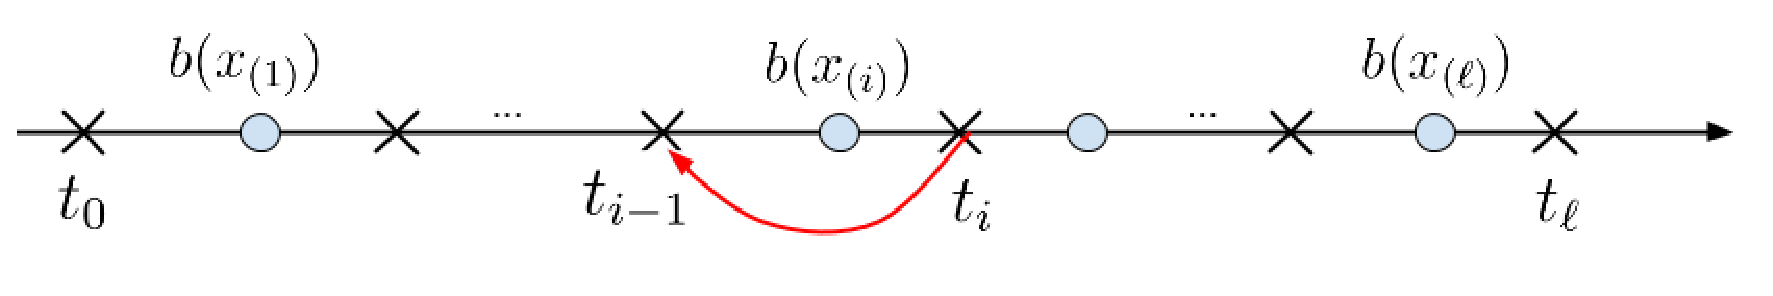
\includegraphics[width=0.8\linewidth]{./img/thresholds.eps}}
		\label{ris:image}
	\end{figure}


	\begin{enumerate}
		\item $y_{(i)} = +1.$ В этом случае классификатор начнет верно классифицировать объект, на котором ранее допускал ошибку, при этом FPR не изменится, а TPR повысится на~$\frac{1}{\ell_+}.$
		\item $y_{(i)} = -1.$ В этом случае классификатор начнет ошибаться на объекте, который ранее классифицировал верно, при этом TPR не изменится, а FPR повысится на  $\frac{1}{\ell_-}.$
	
	\end{enumerate}
	
		\begin{figure}[H]
			\center{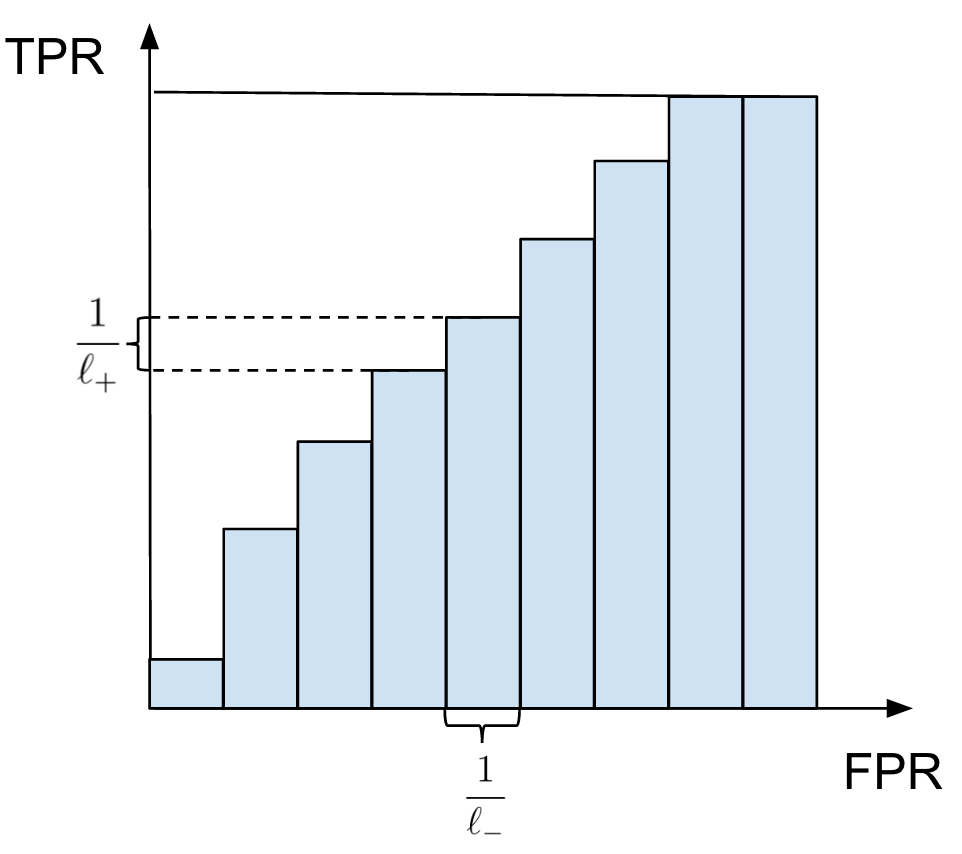
\includegraphics[width=0.6\linewidth]{./img/AUC.eps}}
			\label{ris:image}
		\end{figure}
	
	
	Теперь рассмотрим, как при этом изменяется AUC-ROC. Заметим, что область под ROC-кривой состоит из непересекающихся прямоугольников, каждый из которых снизу ограничен осью FPR, а сверху~--- одним из горизонтальных отрезков, соответствующих второму из рассмотренных случаев. Поэтому каждый раз, когда имеет место второй случай, к текущей накопленной площади под кривой (которая изначально в точке (0; 0) равна 0) добавляется площадь прямоугольника, горизонтальные стороны которого равны $\frac{1}{\ell_-}$, а вертикальные равны $\frac{1}{\ell_+} \sum_{j=i+1}^{\ell} [y_{(j)} = +1]$ (доля уже рассмотренных положительных объектов среди всех положительных), поэтому в этом случае текущее значение AUC-ROC увеличивается на $\frac{1}{\ell_- \ell_+} \sum_{j=i+1}^\ell [y_{(j)} = +1].$
	Итого, финальное значение AUC-ROC можно посчитать~следующим образом:
       \begin{align*}
      \text{AUC} &= \frac{1}{\ell_{+} \ell_{-}} \sum_{i = 1}^{\ell} [y_{(i)} = -1] \sum_{j = i + 1}^{\ell} [y_{(j)} = +1] =\\
       &= \frac{1}{\ell_{+} \ell_{-}}
        \sum_{i = 1}^{\ell} \sum_{j = i + 1}^{\ell} [y_{(i)} < y_{(j)}] =\\
        &= \frac{1}{\ell_{+} \ell_{-}} \sum_{i < j}^{\ell} (1 - [y_{(i)} = y_{(j)}] - [y_{(i)} > y_{(j)}]) =\\
        &= \frac{1}{\ell_{+} \ell_{-}} \sum_{i < j}^{\ell} (1 - [y_{(i)} = y_{(j)}]) - \frac{1}{\ell_{+} \ell_{-}} \sum_{i < j}^{\ell} [y_{(i)} > y_{(j)}] =\\
        &= \frac{1}{\ell_{+} \ell_{-}} \sum_{i < j}^{\ell} ([y_{(i)} \ne y_{(j)}]) - \frac{1}{\ell_{+} \ell_{-}} \sum_{i < j}^{\ell} [y_{(i)} > y_{(j)}] =\\
        &=
        \frac{\ell_{+} \ell_{-}}{\ell_{+} \ell_{-}}
        - \frac{1}{\ell_{+} \ell_{-}}
        \sum_{i < j}^{\ell}
        [y_{(i)} > y_{(j)}]
        = 1
        -
        \frac{1}{\ell_{+} \ell_{-}}
        \sum_{i < j}
        [y_{(i)} > y_{(j)}].
\end{align*}
	Отсюда получаем, что AUC-ROC и доля дефектных пар связаны следующим соотношением:
	$$\text{DP}(b, X) = \frac{2 \ell_- \ell_+}{\ell (\ell -1)} (1 - \text{AUC} (b, X))).$$
	\vspace{0.5cm}
	\end{esSolution}
	
	Заметим, что в случае, когда несколько объектов выборки имеют равные значения $b(x)$, при уменьшении значения порога с $t_i > b(x)$  до $t_{i-1} < b(x),$ где $x$ — один из таких объектов, изменение значений FPR и TPR происходит одновременно, поэтому  соответствующий участок ROC-кривой будет наклонным, а не горизонтальным или вертикальным.
	\begin{vkProblem}
		Пусть даны выборка~$X$, состоящая из 5 объектов, и классификатор~$b(x)$, предсказывающий оценку принадлежности объекта положительному классу. Предсказания~$b(x)$ и реальные метки объектов приведены ниже:
		\begin{align*}
		&b(x_1) = 0.2, \quad  y_1 = -1,\\
		&b(x_2) = 0.4, \quad y_2 = +1,\\
		&b(x_3) = 0.1, \quad y_3 = -1,\\
		&b(x_4) = 0.7, \quad y_4 = +1,\\
		&b(x_5) = 0.05, \quad y_5 = +1.\\
		\end{align*}
		Вычислите AUC-ROC для множества классификаторов~$a(x;t)$, порожденного~$b(x)$, на выборке~$X$.
	\end{vkProblem}
	
	\begin{esSolution}
		В соответствии с процессом построения ROC-кривой, описанным в предыдущей задаче, отсортируем оценки $b(x_i)$ в порядке их неубывания: $(b(x_{(i)}))_{i=1}^\ell = (0.05, 0.1, 0.2, 0.4, 0.7)$. Также составим последовательность реальных меток объектов из этого упорядоченного списка: $(y_{(i)})_{i=1}^\ell = (+1, -1, -1, +1, +1)$.
		
		Построим ROC-кривую (см. рис.~\ref{problem}), откуда $\text{AUC-ROC} = \frac{2}{3}$.
	\end{esSolution}
	\begin{figure}[h]
		\center{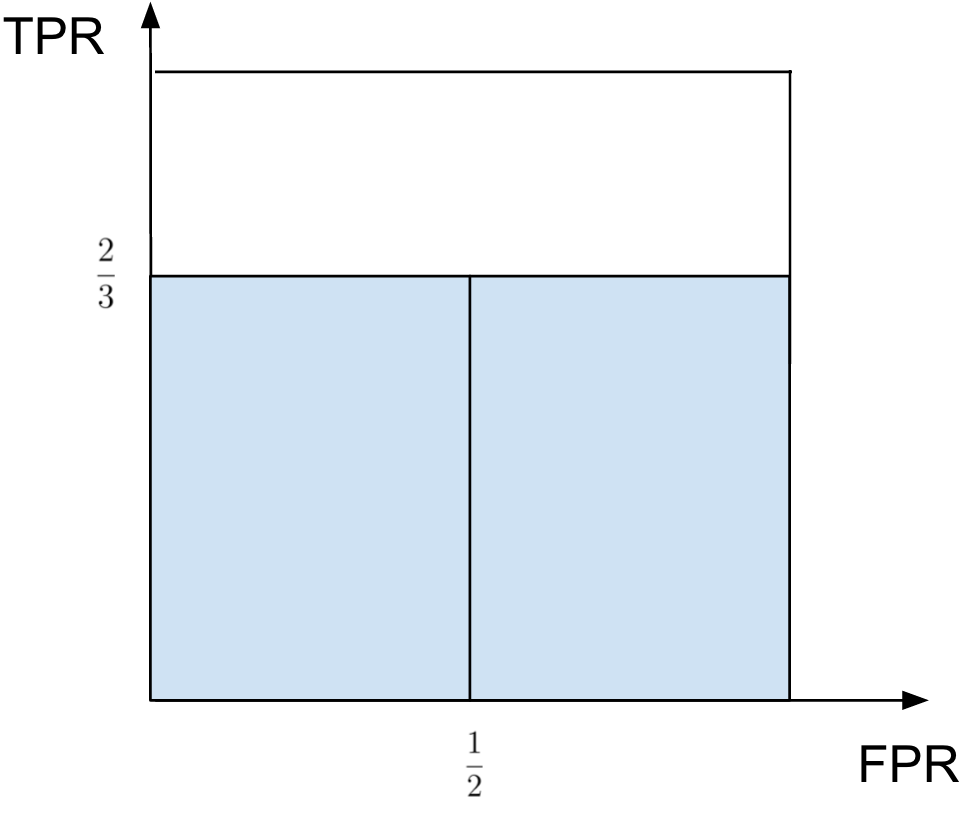
\includegraphics[width=0.4\linewidth]{./img/AUC_problem.eps}}
		\caption{Иллюстрация к задаче 1.2.}
		\label{problem}
	\end{figure}
	
	Заметим, что при вычислении AUC-ROC на некоторой выборке $X$ для итогового классификатора $a(x; t)$ важны не конкретные значения $b(x_i), \, i = \overline{1, \ell},$ а порядок расположения объектов в отсортированном по неубыванию списке $b(x_{(1)}), \dots, b(x_{(\ell)}),$ порожденным алгоритмом $b(x)$. Таким образом, для фиксированной выборки $X$ алгоритм $b(x)$ задаёт перестановку на её объектах, которая в дальнейшем используется при расчёте AUC-ROC.
	
	\vspace{0.5cm}
	
	\begin{vkProblem}
		Пусть $b(x)$ — классификатор, предсказывающий оценку принадлежности объекта $x$ классу +1 таким образом, что для некоторой выборки $X$ он равновероятно выдаёт на её объектах одну из всех возможных перестановок. Чему равно матожидание AUC-ROC этого классификатора?
	\end{vkProblem}
	
	\begin{esSolution}
	Как было показано в задаче 1.1, для AUC-ROC верно
	$$\text{AUC} = \frac{1}{\ell_{+} \ell_{-}} \sum_{i < j}^{\ell} [y_{(i)} = -1] [y_{(j)} = +1],$$
	поэтому
	$$\mathbb{E}\text{AUC} = \frac{1}{\ell_{+} \ell_{-}} \sum_{i < j}^{\ell} \mathbb{E}([y_{(i)} = -1] [y_{(j)} = +1]).$$
	Заметим, что величина $[y_{(i)} = -1] [y_{(j)} = +1]$ принимает значения 0 и 1, поэтому $$\mathbb{E}([y_{(i)} = -1] [y_{(j)} = +1]) = \mathbb{P}(y_{(i)} = -1 , \, y_{(j)} = +1) = \frac{\ell_- \ell_+ (\ell-2)!}{\ell!} = \frac{\ell_- \ell_+}{\ell (\ell-1)}.$$
	Отсюда имеем
	$$\mathbb{E}AUC = \frac{1}{\ell_- \ell_+} \sum_{i<j}^\ell \frac{\ell_- \ell_+}{\ell (\ell-1)} = 
	\frac{\ell (\ell -1)}{2} \frac{1}{\ell (\ell-1)} = \frac{1}{2}.$$
	\end{esSolution}

Итого, можем заметить, что значение AUC-ROC, близкое к $\frac{1}{2},$ означает, что классификатор близок к случайному, тогда как значение, равное 1, означает, что классификатор безошибочно классифицирует объекты при некотором значении порога.

	\begin{vkProblem}
		Пусть $b(x)$ — некоторый классификатор, предсказывающий оценку принадлежности объекта $x$ положительному классу, и при этом AUC-ROC множества классификаторов $a(x;t)$, порожденных $b(x)$, на некоторой выборке $X$ принимает значение, меньшее 0.5.
		Как можно скорректировать прогнозы классификаторов~$a(x;t)$, чтобы они были более осмысленными по сравнению с прогнозами классификатора, выдающего случайные ответы?
	\end{vkProblem}
	
	\begin{esSolution}
%		Заметим, что, поскольку $\text{AUC-ROC} < 0.5$, то ROC-кривая находится под диагональю единичного квадрата.
		
		Для некоторого классификатора $a(x;t)$ рассмотрим классификатор $a^*(x;t)$, выдающий противоположные метки по сравнению с $a(x;t)$, т.е.:
		\begin{align*}
		a^*(x;t) = -a(x;t).
		\end{align*}
		При этом TP и FP на обучающей выборке для некоторого классификатора $a^*(x;t)$ будут принимать следующие значения:
		\begin{align*}
			\text{TP}(a^*(x; t), X) = 
			\sum_{i=1}^\ell [y_i = +1]&[a^*(x;t) = +1] =\\
			&= \sum_{i=1}^\ell [y_i = +1][a(x;t) = -1] = 
			\text{FN}(a(x; t), X),\\
			\text{FP}(a^*(x; t), X) = 
			\sum_{i=1}^\ell [y_i = -1]&[a^*(x;t) = +1] =\\
			&=\sum_{i=1}^\ell [y_i = -1][a(x;t) = -1] = \text{TN}(a(x; t), X).			
		\end{align*}
		Отсюда имеем
		\begin{align*}
			\text{TPR}(a^*(x;t), X) = 
			\frac{\text{TP}(a^*(x;t), X)}{\ell_+} &= 
			\frac{\text{FN}(a(x;t), X)}{\ell_+} =\\
			&=\frac{\ell_+ - \text{TP}(a(x;t), X)}{\ell_+} 
			= 1 - \text{TPR}(a(x;t), X),\\
			\text{FPR}(a^*(x;t), X) = 
			\frac{\text{FP}(a^*(x;t), X)}{\ell_-} &= 
			\frac{\text{TN}(a(x;t), X)}{\ell_-} =\\
			&=\frac{\ell_- - \text{FP}(a(x;t), X)}{\ell_-} 
			= 1 - \text{FPR}(a(x;t), X),			
		\end{align*}
		поэтому классификатор $a^*(x;t)$ будет представлен на плоскости точкой, симметричной точке, отвечающей классификатору $a(x;t)$, относительно точки~$\left(0.5; 0.5 \right)$. 
		
		Рассмотрим ROC-кривую для множества классификаторов~$a(x;t).$ Пусть площадь областей единичного квадрата, находящихся между его диагональю и частями ROC-кривой, расположенных под ней, равна~$S_-,$ а между диагональю и частями ROC-кривой, расположенных над диагональю,~"---~$S_+.$ Тогда AUC-ROC для такой кривой принимает значение $0.5 + S_+ - S_- < 0.5$ (по условию), отсюда~$S_+ - S_- < 0.$
		
		Как было показано ранее, ROC-кривая для множества классификаторов~$a^*(x;t)$ симметрична ROC-кривой для множества классификаторов~$a(x;t),$ а потому для первой кривой область, соответствующая площади~$S_-,$ будет расположена над диагональю единичного квадрата, площади~$S_+$ "--- под диагональю. Отсюда AUC-ROC для множества классификаторов~$a^*(x;t)$ будет принимать значение $0.5 - S_+ + S_- > 0.5,$ а потому прогнозы классификаторов из этого множества  более осмысленны по сравнению со случайным классификатором.
	\end{esSolution}

	\subsection{Прямая оптимизация AUC-ROC}
	\par При обучении модели в бинарной классификации чаще всего решается задача минимизации верхней оценки функционала ошибки:
	\begin{align*}
	Q(a, X) = \frac{1}{\ell}\sum_{i=1}^\ell [a(x_i) \ne y_i] \le \frac{1}{\ell} \sum_{i=1}^\ell \tilde{L}(M_i) \to \min_w
	\end{align*}
	
	Однако иногда возникает необходимость оптимизировать более сложные метрики~"---~в частности, AUC-ROC. Напрямую оптимизировать подобные метрики не представляется возможным из-за их дискретной структуры, однако мы можем использовать трюк с верхней оценкой функционала ошибки и в этом случае. В задаче~1.1 мы показали, что AUC-ROC связан с долей дефектных пар в выборке, поэтому максимизация AUC-ROC равносильна минимизации доли дефектных пар.
	\begin{align*}
	&DP(b, X) = \frac{2}{\ell (\ell - 1)}\sum_{i < j}^\ell [y_i < y_j] [b(x_i) > b(x_j)] =\\  &\frac{2}{\ell (\ell - 1)}\sum_{i < j}^\ell  [y_i < y_j] [b(x_j) - b(x_i) < 0] \le \frac{2}{\ell (\ell - 1)}\sum_{i < j}^\ell  [y_i < y_j] \tilde{L}(b(x_j) - b(x_i)) \to \min_b
	\end{align*}
	Если верхняя оценка $\tilde{L}$ дифференцируема по параметрам модели, то можно оптимизировать такой функционал при помощи градиентных методов.

\end{document}
